\documentclass[12pt]{article}

\usepackage{amsmath, amssymb}
\usepackage{float}
\usepackage{color}
\usepackage{enumitem}
\usepackage[T1]{fontenc}
\usepackage[margin=1in]{geometry}
\usepackage{graphicx}
\usepackage{parskip}
\usepackage{soul}
\usepackage{pgfplots}
\usepackage{cite}

\usepackage{hyperref}
\hypersetup{
    colorlinks=true,
    citecolor=black,
    linkcolor=blue,
    filecolor=magenta,      
    urlcolor=cyan,
}

\graphicspath{
    {img/}
}

\begin{document}
    
\begin{titlepage}
    \centering
    \vspace*{2.5cm}
    
    \Huge
    \textbf{Project Proposal} \\
    
    \huge
    \textbf{Segmentation in Medical Imaging}
    
    \vfill
    
    \LARGE
    Zhaotian Fang (z23fang) \\
    Zhaotian Fang (z23fang) \\
    Zhaotian Fang (z23fang) \\
    \today \\
    CS221 \\
    Autumn 2019 \\
    Stanford University
\end{titlepage}

\section{Introduction}
In recent years, there has been renewed interest in accurate segmentation of magnetic resonance (MR) images, especially for the human brain. In this task, there are two focus areas: neuroanatomy segmentation on the whole brain as well as anomaly detection and segmentation on the lesion or tumor areas. The neuroanatomy segmentation forms the foundation for volume and shapes analyses to track the progression of diseases over time. Moreover, it provides labelling of brain structures such as the white matter, cortex, hippocampus, etc. to help neuroscience studies. The brain MR images are often used for pathological diagnosis. The accurate detection and segmentation of brain lesions or tumors are even more critical.

\section{Related Work}
Since manual segmentation of brain neuroanatomy and lesions is time-consuming, there has been a plethora of efforts in automating and accelerating the process. In terms of unsupervised approaches for brain neuroanatomy segmentation, the most commonly used is a software tool named FreeSurfer \cite{freesurfer}. There has been an abundance of follow-up research on multi-atlas registration and label fusion (MALF) (citation here). However, these techniques are computationally intensive, taking several hours to produce a single segmentation result. As for brain lesion segmentation, a MATLAB toolbox named Lesion Segmentation Tool (LST) is usually used to identify lesion areas. As a post-processing step, the resulting lesion segmentations are then manually adjusted by radiologists for better precision.

In attempts to improve on the efficiency of brain anatomy segmentation and lesion segmentation, supervised Convolutional Neural Network (CNN) based approaches have been emerging over the past few years. However, these methods are faces two main constraints on performance. First, these supervised models require an extensive amount of high-quality segmentation labels. These labels are usually created manually and thus hard to obtain. Secondly, these models primarily operate on similar applications base on the dataset they were trained on. Due to the high cost associated with label acquisition in addition to hardware limitations, high quality MRI datasets appropriate for training neural networks are limited. As a result, supervised approaches like CNNs struggle with generalization. Therefore, there is a need to find a generalizable model to efficiently segment the brain MR images in an unsupervised manner.

In the medical field, there have been a few attempts to use deep learning with the object to achieve unsupervised segmentation. Stacked denoising autoencoders were used as a pre-training step before supervised learning. (Citations) Generative models such as the AnoGAN framework and Variational Autoencoders were deployed to learn healthy brain images, assuming that when fed with brain images with anomalies, the network will be able to classify the image as abnormal. An effort was made to combine the above-mentioned frameworks into what is called AnoVAEGAN to segment brain lesions in an unsupervised way. However, these approaches are still rely on large sets of high-quality and healthy brain images to learn effectively.

\section{Method}
% Define the input-output behavior of the system and the scope of the project.

Lately, in the computer vision field, a novel method was proposed by Ji Xu et al. to use invariant information clustering (IIC) for unsupervised image classification and segmentation.  This method uses a clustering technique where it maximizes the mutual information between the class assignments of each pair and can directly output labelings on each pixel. In this project, we propose a technique similar to IIC to provide both neuroanatomy segmentations and lesion segmentations on brain MR images in an unsupervised manner.

The input to our system is a slice of a brain MRI. The output to our system consists of two segmentation masks: one neuroanatomy semantic mask decomposing the brain image into its anatomical components, and another lesion binary mask indicating the presence of brain tumors.

\section{Challenges}
% What are the challenges? Which topics (e.g., search, MDPs, etc.) might be able to address those challenges (at a high-level, since we haven't covered any techniques in detail at this point)?
% challenges be what is difficult about solving this problem without the use of AI, or should it be more about what problems might arise when trying to implement our methods?
In general the task of image segmentation is very hard. Traditional image segmentation comprise of various edge-based and region-based methods \cite{segmentation_survey}. However, these methods are not robust and do not generalize well across different datasets. In terms of the topics covered in class, deep learning based methods like CNNs will be useful since they have been proven in research to work well across many different domains.

During the implementation of our system, one challenge we face is dealing with the uncertainty around whether we propose will be able learn from brain MRIs. Although IIC has shown to work with image distributions occuring in nature, it's unclear how well the method will transfer to MR images. 

\section{Dataset}
% Collect some preliminary data, and give concrete examples of inputs and outputs.
Out data will mainly come from three sources:
Human connectome project
MS lesion segmentation challenge 2008
data from MGH

\begin{figure}[htbp!]
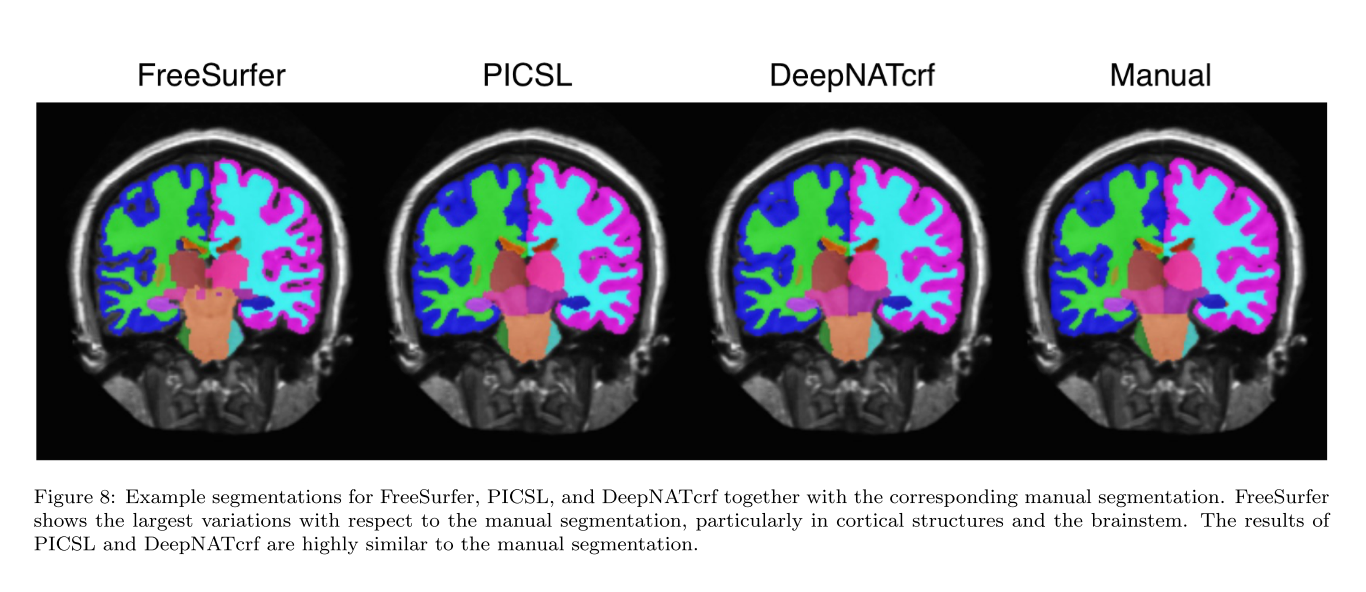
\includegraphics[width=\textwidth]{ana_seg1.png}
\end{figure}

\begin{figure}[htbp!]
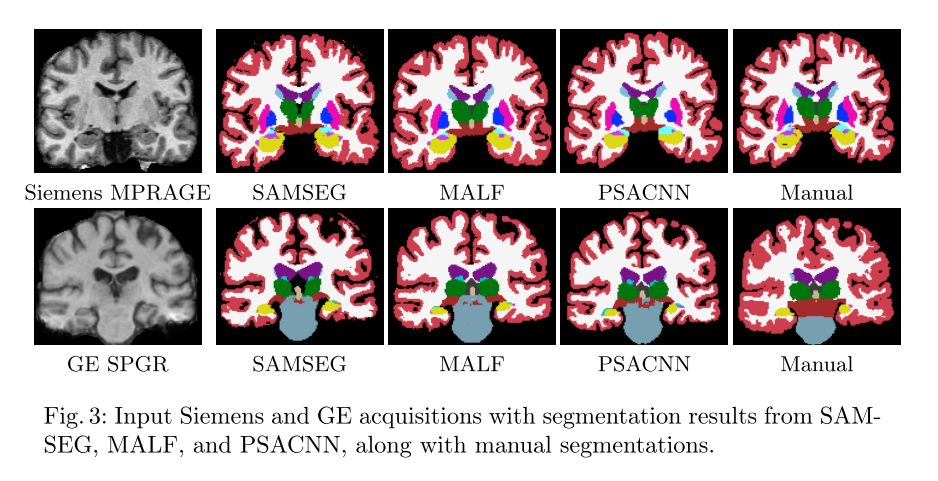
\includegraphics[width=\textwidth]{ana_seg2.png}
\end{figure}

\begin{figure}[htbp!]
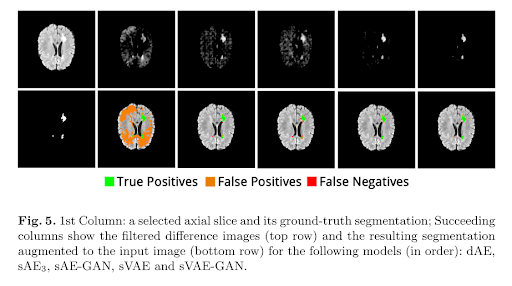
\includegraphics[width=\textwidth]{tumor_seg.png}
\end{figure}

\section{Baseline \& Oracle}
% Implement a baseline and an oracle and discuss the gap
The baseline for our system is a combination of anatomy segmentation results from FreeSurfer and the lesion segmentation results from LST. The Oracle of the system is naturally the segmentation labels provided by the radiologists. The gap between them are… 

Baseline 
Whole brain segmentation:  FreeSurfer (TOO HARD????)
Lesion Segmentation: https://www.applied-statistics.de/lst.html

Oracle:
Whole brain segmentation:  Radiologist???
Lesion Segmentation: Radiologist

\section{Evaluation}
% What is your evaluation metric for success?
In order to evaluate the quality of the segmentation we can use a variety of different metrics including the Dice Coefficient, and mean IOU. For some complicated structures, we may need to have some radiologists to evaluate the results of different methods (objective scoring). 

\bibliographystyle{IEEEtran}
\bibliography{proposal}

\end{document}
